\documentclass[12pt]{article}
\input{/Users/circle/Documents/博一下/homework/setting.tex}
\setcounter{secnumdepth}{2}
\usepackage{bm}
\usepackage{autobreak}
\usepackage{amsmath}
\setlength{\parindent}{2em}
\graphicspath{{../}}

%pdf文件设置
\hypersetup{
	pdfauthor={袁磊祺},
	pdftitle={统计力学及应用作业1}
}

\title{
		\vspace{-1in} 	
		\usefont{OT1}{bch}{b}{n}
		\normalfont \normalsize \textsc{\LARGE Peking University}\\[1cm] % Name of your university/college \\ [25pt]
		\horrule{0.5pt} \\[0.5cm]
		\huge \bfseries{统计力学及应用作业1} \\
		\horrule{2pt} \\[0.5cm]
}
\author{
		\normalfont 								\normalsize
		College of Engineering \quad 2001111690  \quad 袁磊祺\\	\normalsize
        \today
}
\date{}

\begin{document}

\input{setc.tex}

\maketitle

\section{1}

\cref{fig:1} 为使用 Matlab 的 \texttt{rand} 函数产生的概率分布图.可以发现正反面的概率都趋于$0.5$.

\begin{figure}[htp]
	\centering
	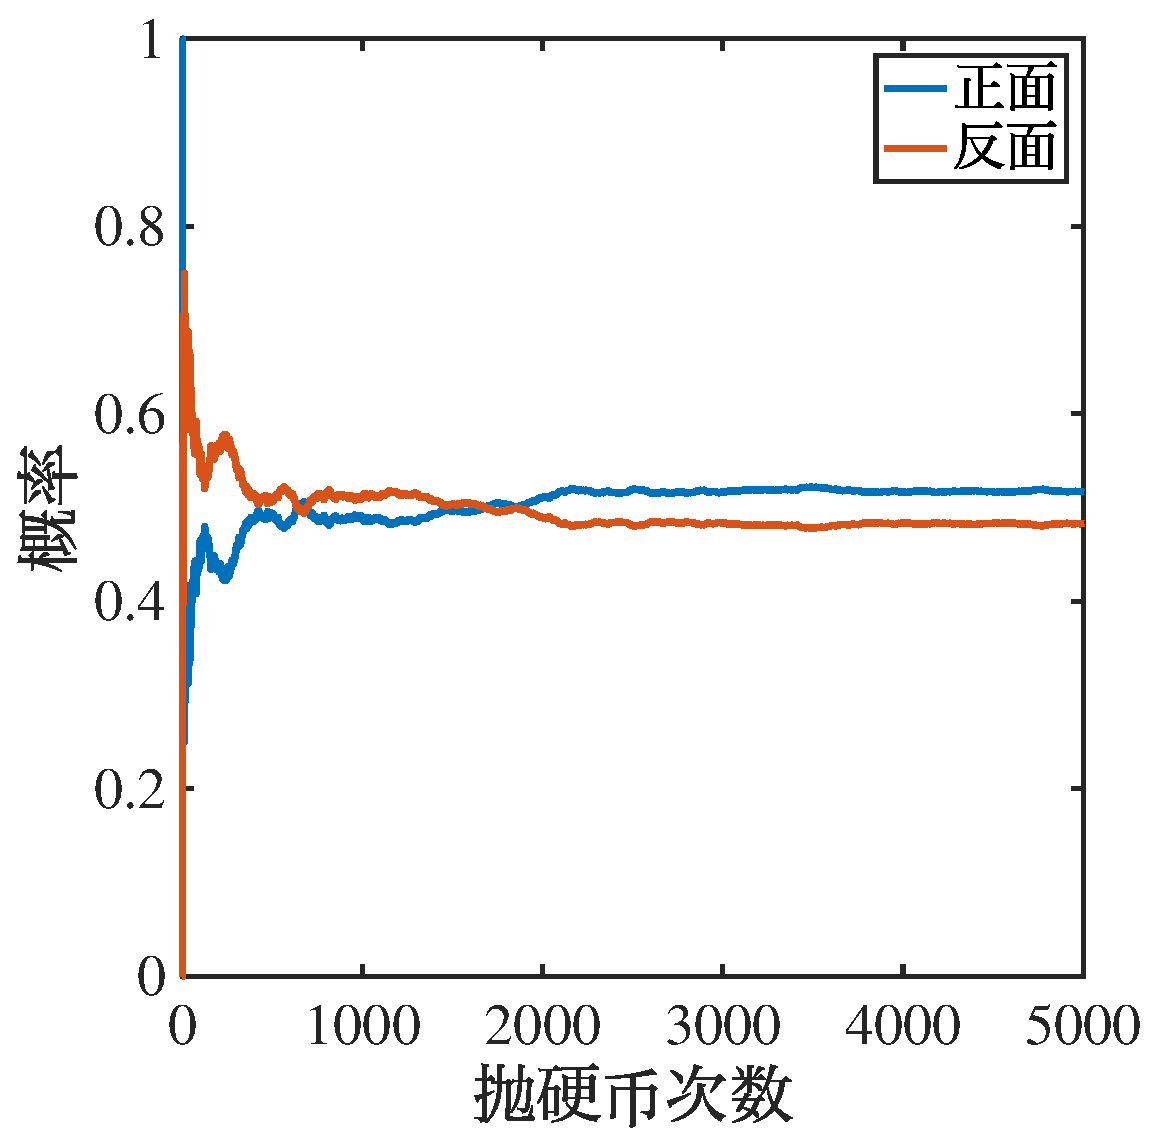
\includegraphics[width=7cm]{posi1.eps}
	\caption{正面和反面的概率.}
	\label{fig:1}
\end{figure}


\section{2}

\cref{fig:2} 为使用同余伪随机数方法产生的概率值.这里使用的是\cite{10.5555/42249}中给出的数据:

\lstset{language=Matlab}
\begin{lstlisting}
im = 714025;
ia = 4096;
ic = 150889;
\end{lstlisting}

然后任意给出两组初值来计算概率,正面和反面的概率和为1.

\begin{figure}[htp]
	\centering
	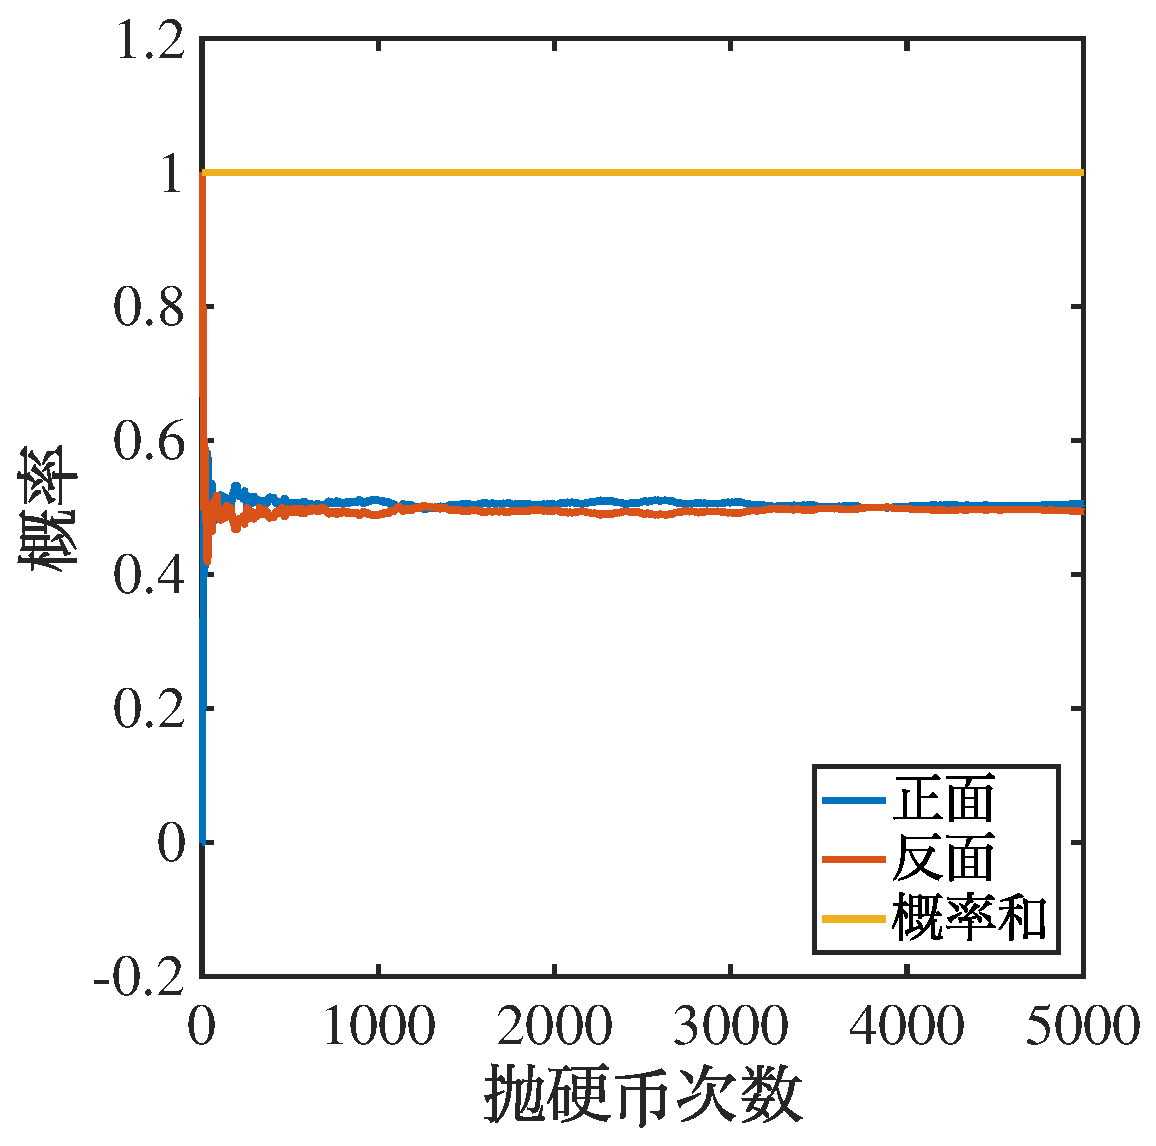
\includegraphics[width=7cm]{posi2.eps}
	\caption{正面和反面的概率.}
	\label{fig:2}
\end{figure}

\cref{fig:3} 为使用同余伪随机数方法计算同时抛两个银币同时为正,同时为负,一正一负的概率,可以发现前两个概率都趋于0.25,而最后一个概率趋于0.5.

\begin{figure}[htp]
	\centering
	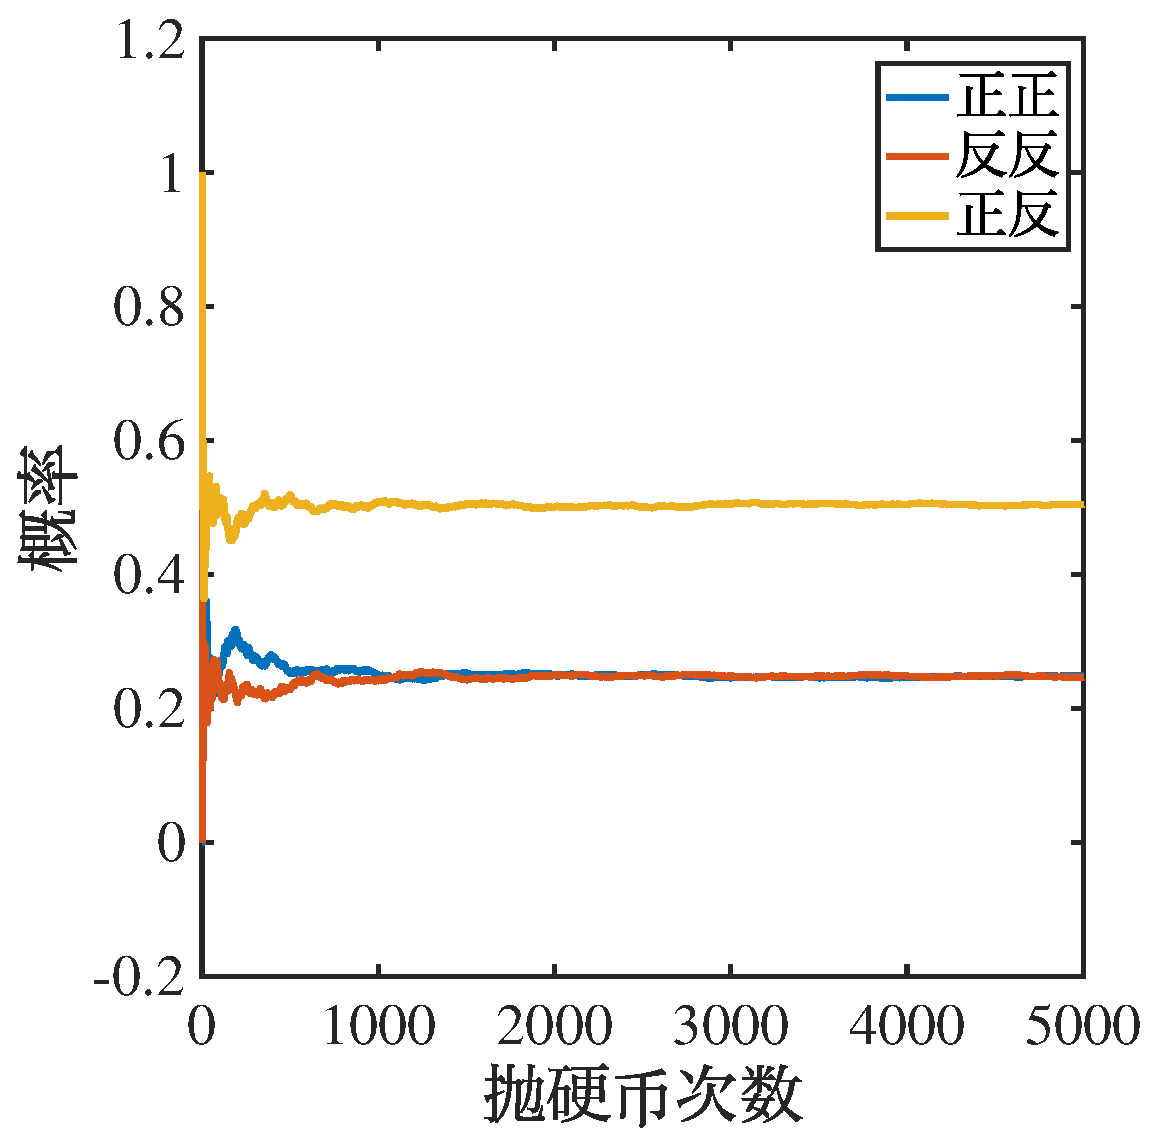
\includegraphics[width=7cm]{posi3.eps}
	\caption{正正,反反,正反的概率.}
	\label{fig:3}
\end{figure}

\cref{fig:4} 为正正,反反,正反的概率与期望的差.可以发现三者的误差都趋于0.

\begin{figure}[htp]
	\centering
	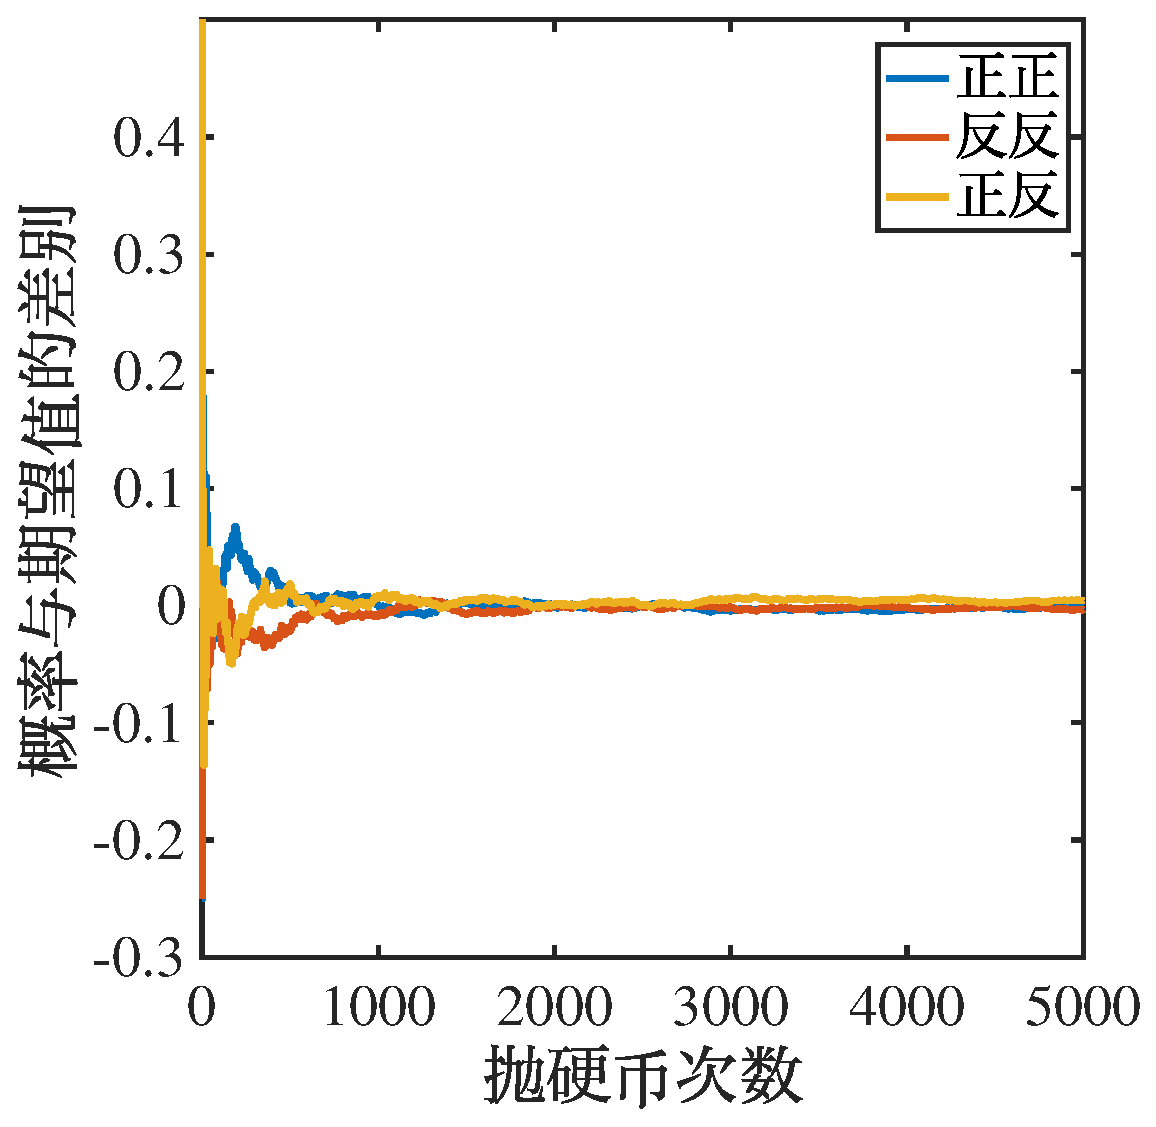
\includegraphics[width=7cm]{posi4.eps}
	\caption{正正,反反,正反的概率与期望的差.}
	\label{fig:4}
\end{figure}




% \nocite{*}

\input{bib.tex}

\end{document}
